\chapter{Spatial Transformer Networks}

The use of spatial transformers results in models which learn invariance to translation, scale, rotation and more generic warping, resulting in state-of-the-art performance on several benchmarks, and for a number of classes of transformations.

\begin{figure}[h]
  \centering
  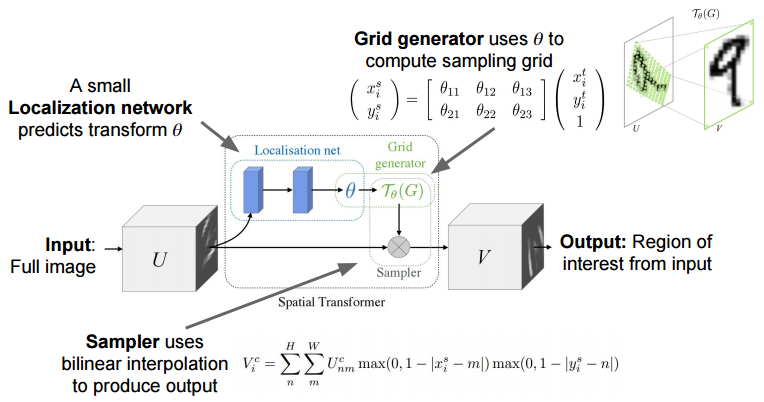
\includegraphics[width=0.8\textwidth]{Images/spatial_transformer_networks/2.png}
  \caption{Spatial Transformer Networks}
\end{figure}

We would like a function that given a continuous box coordinates cropped the input image. The problem is that it is not possible to crop in a continuous way because we are constraint, at least, by pixels.

The idea is to have a function that maps output pixels coord to input pixels coord. This function is deferentiable w.r.t the affine parameters $\theta$.

With this function, the network will attend to input regions by predicting $\theta$.

\begin{figure}[h]
  \centering
  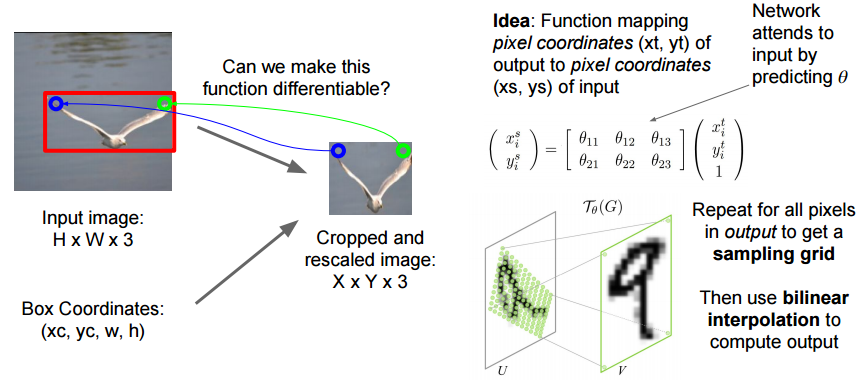
\includegraphics[width=0.8\textwidth]{Images/spatial_transformer_networks/1.png}
  \caption{continious coordinates}
\end{figure}

They put the info explained on top row in a self contained module which they call "Spatial Transformer" which is divided in three parts:
\begin{itemize}
\item Localisation net: Outputs the affine parameters $\theta$.
\item Grid Generator: Use $\theta$ to compute the sampling grid
\item Sampler: With bilinear interpolation produces outputs.
\end{itemize}

Notice that all this modules are continuous and differentiable.

\begin{figure}[h]
  \centering
  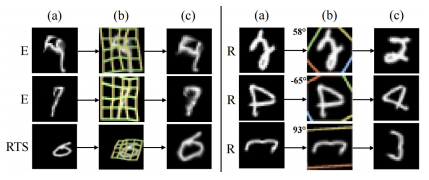
\includegraphics[width=0.8\textwidth]{Images/spatial_transformer_networks/3.png}
  \caption{Deformation examples}
\end{figure}